\begin{tikzpicture}[scale=0.6]
  \usetikzlibrary{calc}
  \tikzstyle{branch}=[color=black, line width=4pt, line join=miter]
  \coordinate (origin) at (0,0);
  \coordinate (bl) at (-6,0);
  \coordinate (S1) at (5,9);
  \coordinate (S2) at (5,6);
  \coordinate (B1) at (0,4);
  \coordinate (B2) at (0,1);
  \node[anchor=west,outer sep=1ex] (Seq1) at (S1.east) {{ACCGTATCGCCA}};
  \node[anchor=west,outer sep=1ex] (Seq2) at (S2.east) {{ACCG\textcolor{red}{GC}TCG\textcolor{red}{G}CA}};
  \coordinate (R1) at (S1 |- B1);
  \coordinate (R2) at (S2 |- B2);
  \coordinate (Bmid) at ($(B1)!0.5!(B2)$);
  \coordinate (Smid) at ($(S1)!0.5!(S2)$);
  \coordinate (L) at (bl |- Bmid);
  \node[anchor=west] (R1i) at (R1.east) {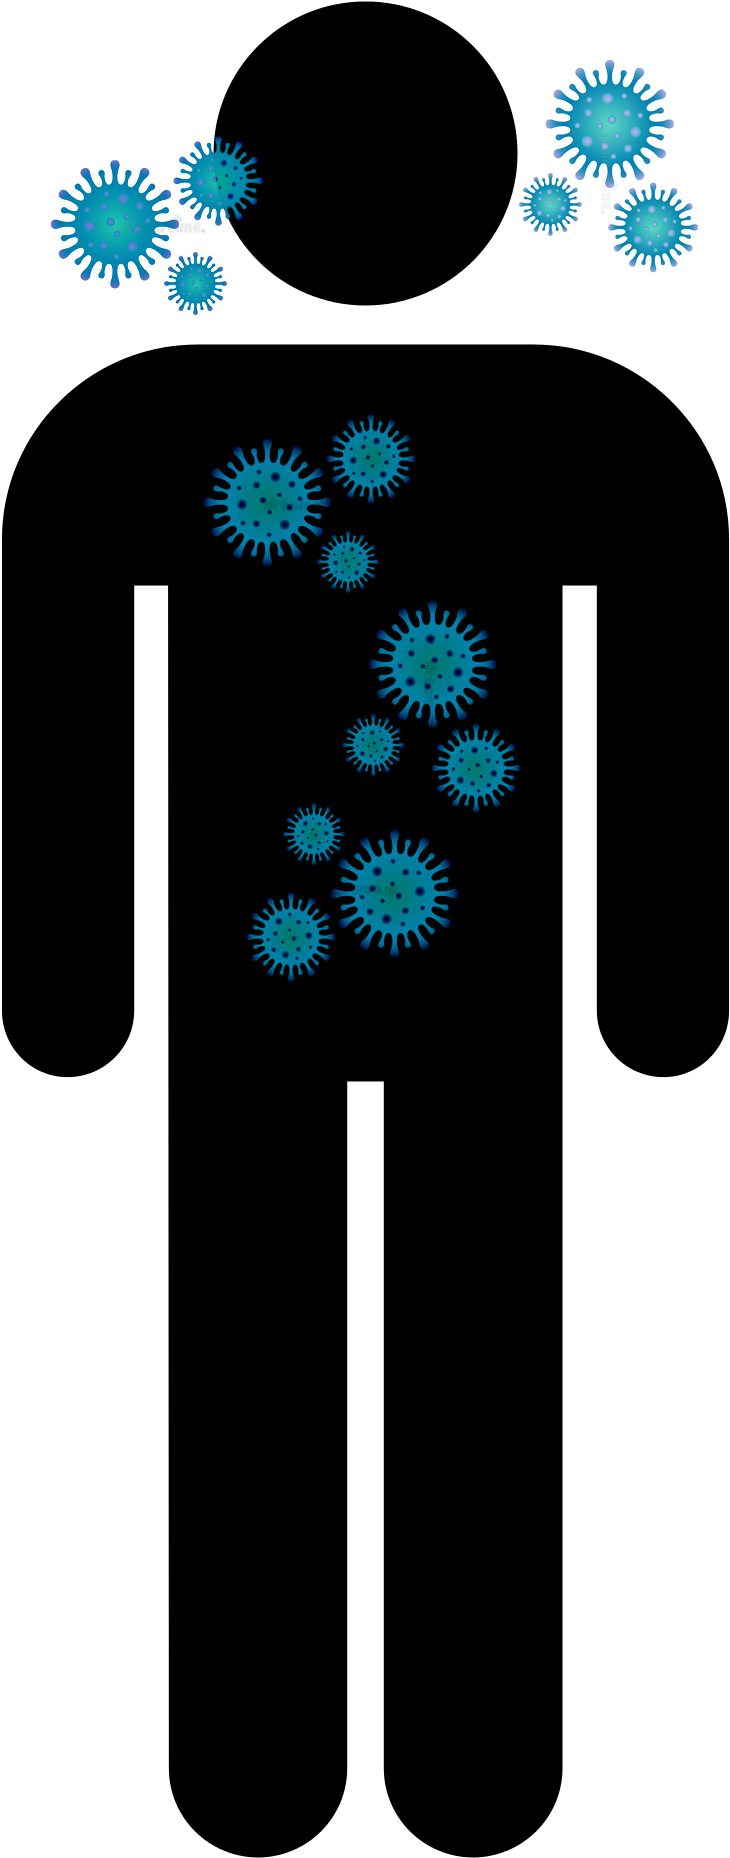
\includegraphics[height=36pt]{infected}};
  \node[anchor=west] (R2i) at (R2.east) {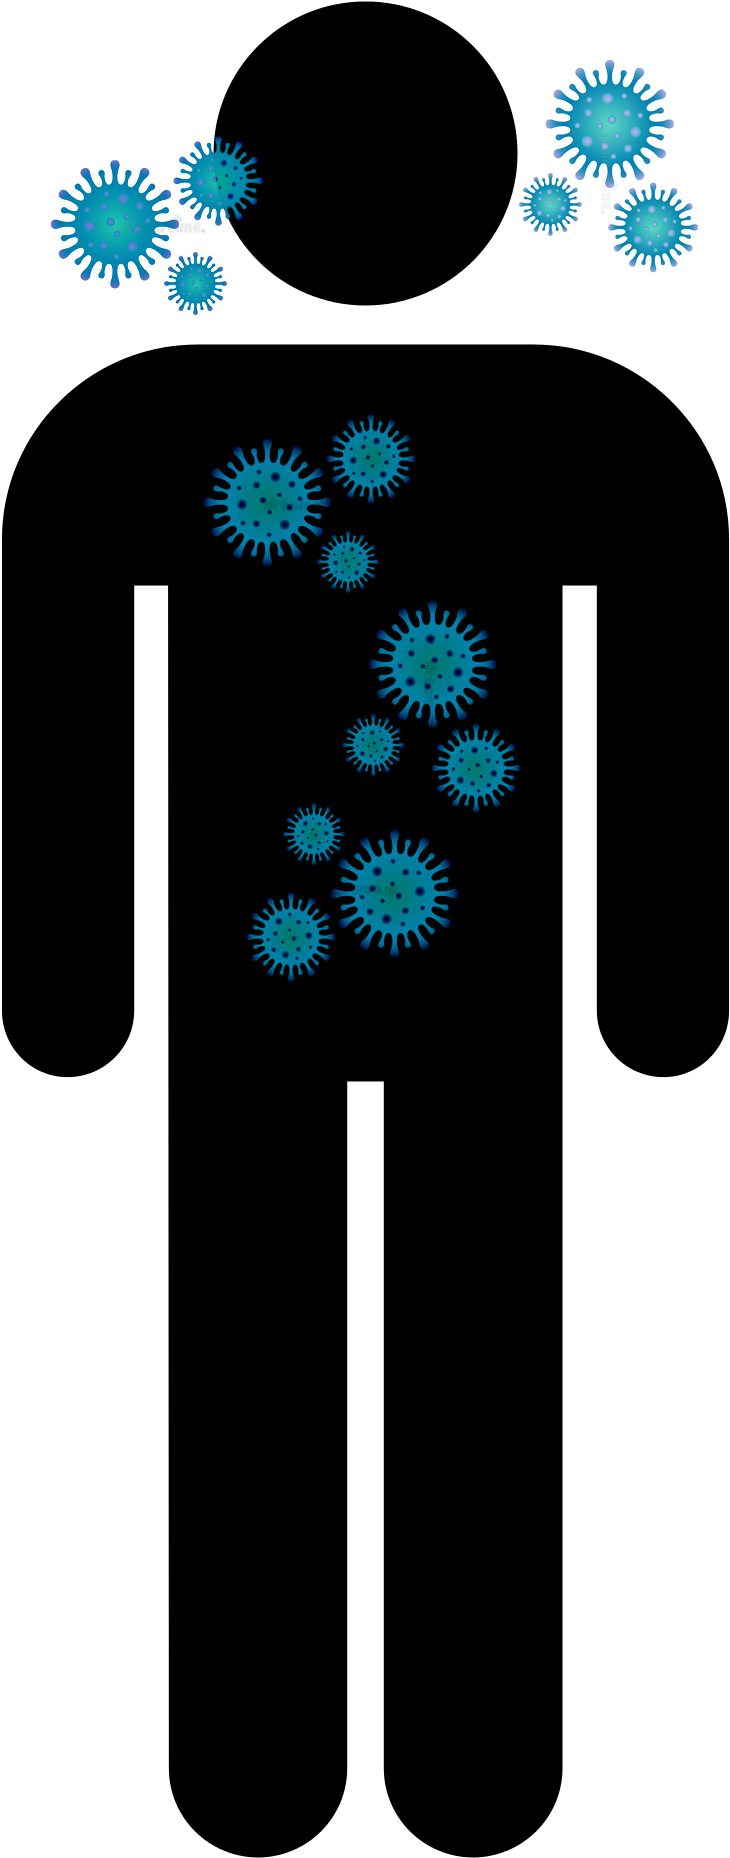
\includegraphics[height=36pt]{infected}};
  \draw[branch] (R1i.west) -- (B1) -- (Bmid) -- (L) (R2i.west) -- (B2) -- (Bmid);
  \node[anchor=east] (Li) at (L.west) {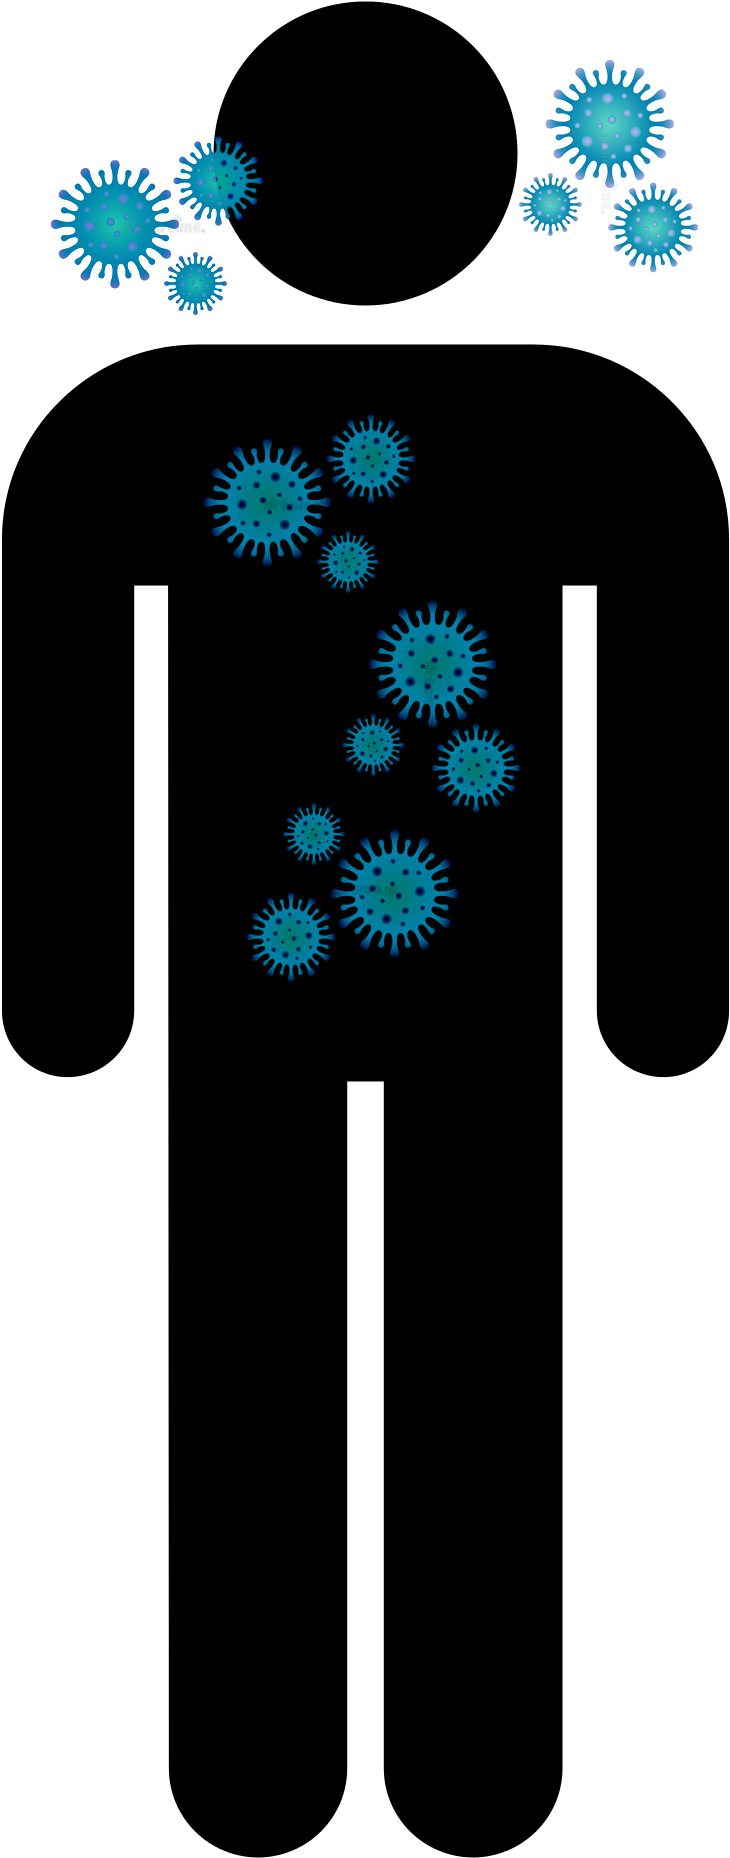
\includegraphics[height=36pt]{infected}};
  \draw[branch,color=blue] (S1) -- (origin |- S1) -- (origin |- S2) -- (S2);
  \node[anchor=east,outer sep=2ex] (lab1) at (L.west) {\parbox[t]{72pt}{\raggedright Transmission tree}};
  \node[anchor=east,outer sep=2ex] (lab2) at (L.west |- Smid) {\parbox[t]{72pt}{\raggedright Pathogen genealogy}};
  \coordinate (tc) at ($(origin|-Seq1.north)+(0,1em)$);
  \draw[very thin,color=gray] (origin) -- (tc);
  \node (tlab) at ($(Seq1.east|-origin)+(1em,0)$) {$t$};
  \draw[thin,->,>=latex] (bl) -- (tlab);
\end{tikzpicture}
